%1234567890123456789012345678901234567890123456789012345678901234567890123456789
\chapter{Introduction}
 
% Our problem (=dynamic motor skills) is important
Learning highly dynamic motions of athletes has been one of the greatest
challenges for humanoids, from a virtual character in simulation to a real
robot with hardware.
The learned dynamic motor skills allow humanoids to generate more agile,
efficient, and responsive motions that are useful in many applications.
One notable benefit is that a humanoid can overcome obstacles as swiftly and
efficiently as possible using only its body.
A robot in a disaster place is likely to encounter the uneven
terrains and discontinuous gaps, which cannot be explored by regular
locomotion without dynamic motions such as jumping or falling.
In addition, dynamic motor skills maximize capability of humanoids
under the given torque and joint limitations.
If a virtual character in a sports game cannot execute athletic movements
of elite sports players, a game will be boring and not appealing to users.
A game character can further adapt the acquired skills to the
environment changes or user interactions under the valid physical assumptions,
such as minimizing energy consumption.
The advantages of highly dynamic motor skills lead to the
development of techniques for learning physics-based motion controllers
in the various areas in academia and industry.


% I will solve virtual and real both, to get the benefits
Virtual characters and real robots are two main subjects of motor control
problems in computer graphics and robotics, which have both common and
different properties.
To name a few, control problems in both areas have non-linear
objective function, under-actuated characters, high-dimensional
control parameters.
There are also different assumptions and limitations
on sensors, actuators, contacts, control mechanisms, and so on.
It is often possible to apply the existing principles and
algorithms developed in one domain to the other and expedite the
design process of the controller, 
if they are robust enough to handle different assumptions.
For instance, a virtual simulation of a robot is often used as a testbed for
developing hardware compatible controllers due to the expensive cost and
time-consuming trials [,,].
The techniques that are designed to control noisy hardware systems 
can be applied to virtual characters for creating more robust controllers.
In this dissertation, I will develop control techniques for both virtual and
real humanoids to demonstrate how the algorithms in two different systems can
benefit each other.

% Dynamic motor skills itself is very difficult
Highly dynamic motor skills are difficult tasks for humanoids.
Execution of dynamic motions accompanies abrupt accelerations and decelerations
of momentum, frequent changes of contacts, and explosive usage of torques near
limitations.
Therefore, control becomes a very sensitive problem because small errors can
quickly accumulate and generate a disastrous result to the humanoid, such as
loosing it balance and hitting the ground.
One of very challenging motions is safe falling of a humanoid, which is 
a fundamental motor skill that protects the subject from severe
injuries and connects the previous and next actions for fluent transitions.
A falling motion requires very accurate control because a robot must decelerate
huge vertical momentum within a very short time window, and a minor failure
will cause huge damage to the body parts.
In addition, a wide range of initial conditions must be considered 
for robustness because falling can be initiated by unexpected situations.
The development of falling controllers will make virtual 
characters and robots to execute motions safely and smoothly,
and its principles can be applied to the other highly dynamic motions
with huge momentum.

% The first difficulty: the design of the controller
There are several issues when a user develops physics-based controllers
for difficult dynamic motor skills.
The first problem arises when the user designs objectives, control 
mechanisms, and control parameters, which require a lot of prior knowledge.
Since a large portion of controller designs remains unknown until testing
the implementation, the design process is often driven by trial-and-errors.
This can be very tedious and time-consuming, especially in the traditional
monolithic optimization setting that may take several hours to days.
Thus, it is important to develop a simple and intuitive design process
that allows the user to train controllers within a short amount of time.
An iterative learning can be more efficient due to 
short feedback loops that can easily test and modify the controller,
and more intuitive because it is similar how human learn motor skills
through progressive process of coaching and practicing.

% The second difficulty (optimization) and our approach
Optimizing control parameters for dynamic motions is another time-consuming
step that requires a lot of computing power.
Typically, whole-body dynamic tasks typically have a cost function
that is multimodal, non-linear, non-convex, and discontinuous due to 
an under-actuated system and discrete contacts.
Further, control parameters are likely to be in a high dimensional
space with small feasible regions that does not generate undesired behaviors.
These difficulties often require the most robust optimization algorithm.
In computer animation, a robust black-box sampling-based method, 
Covariance Matrix Adaption Evolution Strategy (CMA-ES) [], has been frequently
applied to discontinuous control problems, such as biped locomotion [],
parkour-style stunts[], or swimming [].
However, CMA-ES is not the most effective algorithm for
optimizing dynamic motor skills when they have small feasible regions
or high-dimensional control space due to the parametization.
This motivated me to work on improving the performance of the baseline
algorithm, CMA-ES, for more difficult tasks with many user constraints
I further extend CMA-ES for a parametrized motor skill, which is essential
for operating a robot in the unpredictable environment.

% The third difficulty (simulation bias) and our approach
Unlikely the optimization for virtual characters,
a control policy search for hardware with many trials is often infeasible
because conducting hardware experiment can be expensive and time-consuming.
Moreover, an execution of a bad controller on a robot can potentially cause
disastrous damage to the robot and enormous cost to repair.
To reduce the number of trials on the hardware, a virtual simulation 
is used as a practical solution that provides a fast and safe evaluation
of the control parameters.
However, it suffers from \emph{simulation bias} in which
controllers developed for a virtual character do not work on hardware due
to differences in the two systems.
The \emph{simulation bias} is hard to explicitly model because it can
be caused by many reasons, such as different mass-distributions, sensor 
and actuator noises, command delays, and more.
Therefore, a data-driven model-based policy search, which iteratively 
updates the simulation using collected hardware data, is a promising method 
to model the simulation bias, which will be discussed in this dissertation.

% Identify three categories problems.
I will present the following identified problems for developing 
controllers for highly dynamic motor skills.

\section{Falling Strategies for Humanoids}
% Introduction on the falling - Motivation, Description, Goal
Highly dynamic motions often accompany the abrupt momentum changes, which can
cause large contact forces to characters.
Therefore, how to manage falls is a fundamental motor skill to reduce damages
to humanoids and achieve fluent transitions between motor skills.
In this dissertation, I will discuss two different falling scenarios, 
for  virtual and real humanoids.
For a virtual character, I will describe a general controller that allows the character to fall from a wide range of heights and initial speed,
which are inspired by falling of traceurs.
For a real robot, a general falling strategy for handling various 
external perturbations is introduced, which is feasible to be
executed by actual hardware.
The effectiveness of the presented strategies will be validated in physics
simulation, and experimentally tested on a small-size humanoid.

\subsection{Falling and Landing Motion Control for Virtual Characters}
% Goal, Method (Strength), Verification + Image

In Chapter 3, I will show how to create an on-line controller for generating 
agile and natural falling motions of the virtual character that can land from 
various heights and velocities.
The goals of the controller are to reduce the joint stress at the impact and
get back on its feet to prepare the next action.

\begin{wrapfigure}{r}{0.5\textwidth}
 \vspace{-25pt}
  \begin{center}
    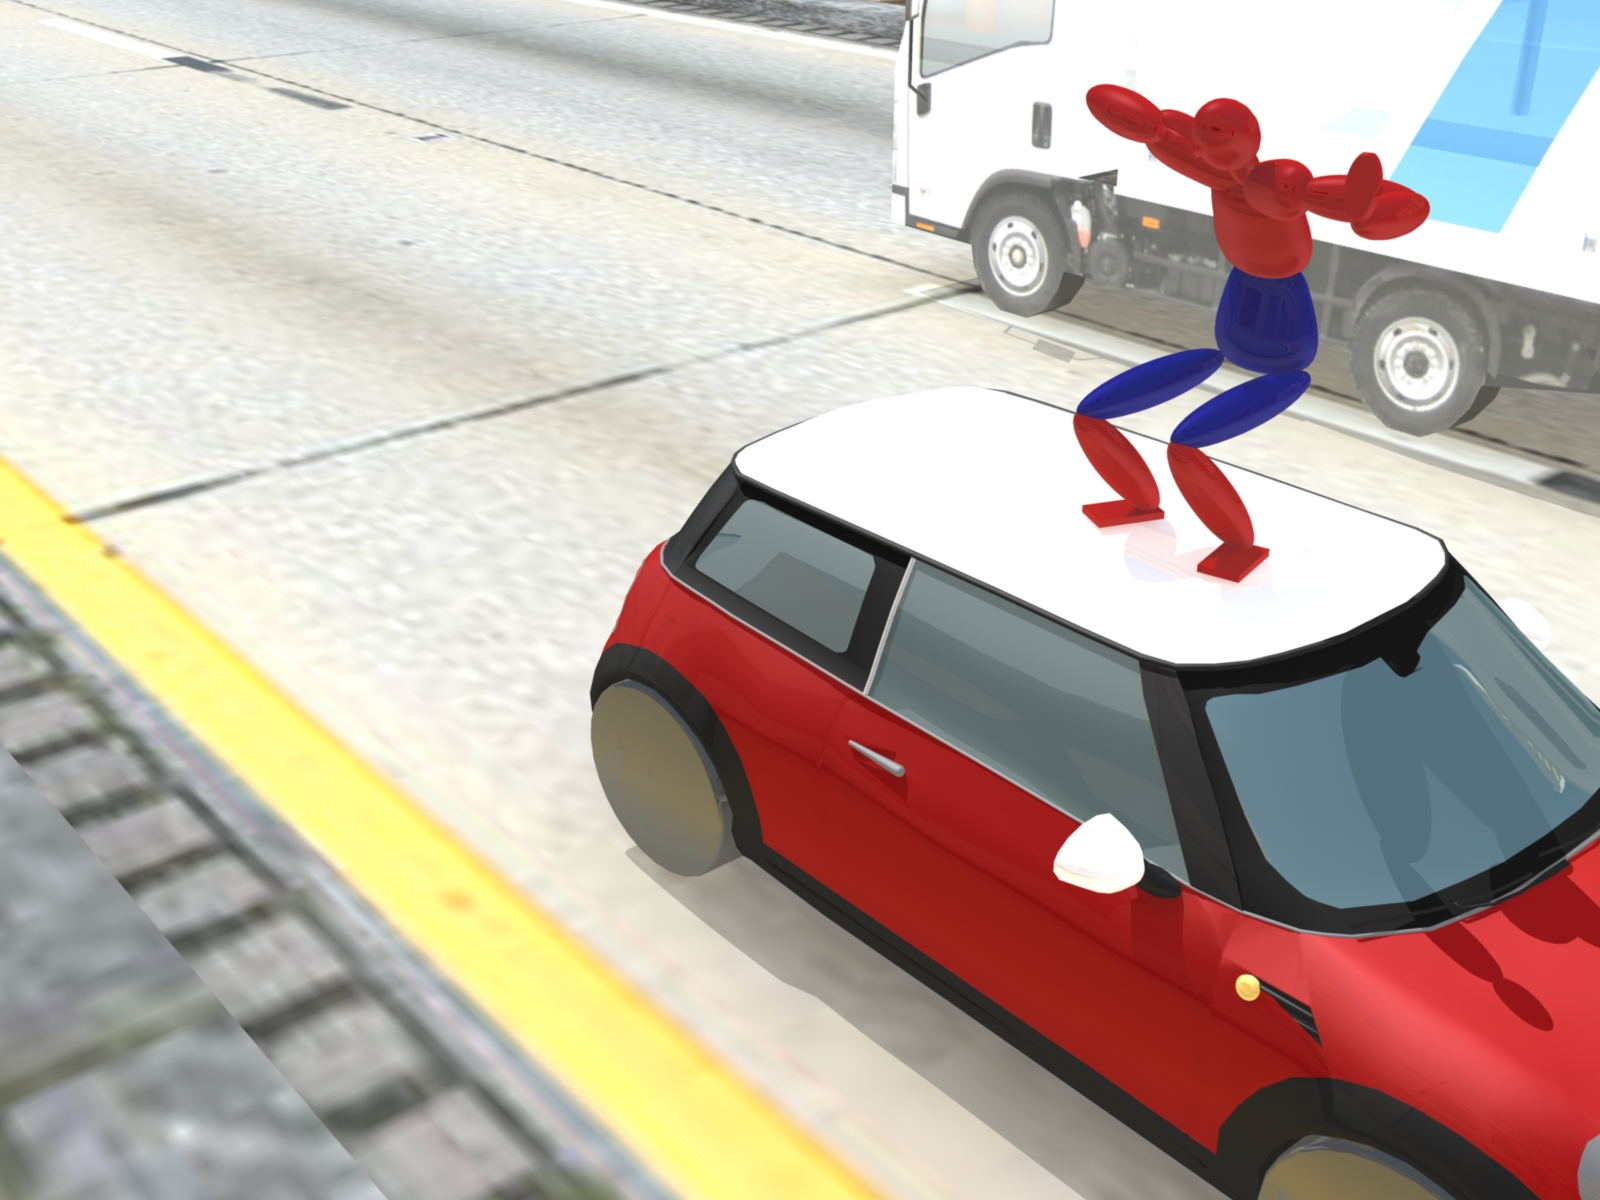
\includegraphics[width=0.48\textwidth]{images/intro_landing.jpg}
  \end{center}
   \vspace{-25pt}
  \caption{A falling motion of Parkour.}
  \label{fig:intro_landing}
   \vspace{-10pt}
\end{wrapfigure}
Inspired by falling skills of Parkour(\figref{intro_landing}), 
I formulate the falling problem
with three phases, \emph{airborne}, \emph{impact}, and \emph{rolling}
based on the contact states.
First, two sub-controllers are designed for the \emph{airborne} and
\emph{rolling} phases and a regression analysis is conducted to find 
an optimal landing angle that can connect two sub controllers at the
\emph{impact} phase.
I will demonstrate that the motion generated by the proposed controller
induces smaller joint stress, which is still four times lower than a rag-doll
motion at the worst cases.



\subsection{Multiple Contact Planning for Humanoids}
\begin{wrapfigure}{l}{0.5\textwidth}
 \vspace{-25pt}
  \begin{center}
    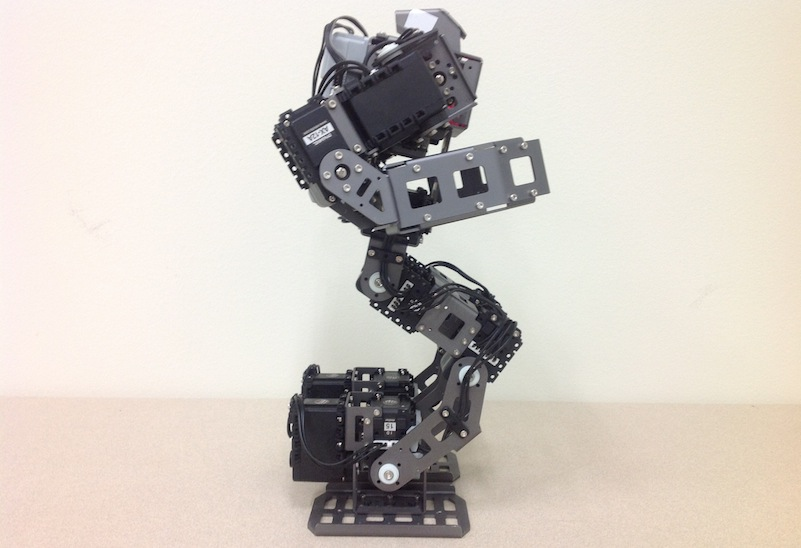
\includegraphics[width=0.48\textwidth]{images/intro_hardware.jpg}
  \end{center}
   \vspace{-25pt}
  \caption{Hardware of BioloidGP robot.}
   \vspace{-10pt}
  \label{fig:intro_hardware}
\end{wrapfigure}
% Goal, Method (Strength), Verification + Image
Chapter 4 will describe a general algorithm which plans for appropriate 
responses to a wide variety of falls, from a single step to recover a gentle nudge, to a rolling motion to break a high-speed fall.
Our multiple contact planning provides a unified framework
that can represent many existing falling techniques [,,].
Then, I will show how to efficiently optimize the multiple contact falling
strategy to the given initial state using a simplified model and dynamic 
programming.
Finally, various scenarios will be tested on simulated humanoids and the
actual hardware (\figref{intro_hardware}) to show that our algorithm plans
various falling strategies with different contact sequences.

\section{Learning of Dynamic Controller for Characters}
% Introduction on the learning - Motivation, Description, Goal
Teaching a physically simulated character a new motor skill requires 
a lot of efforts from the controller designer, from the design of the control 
mechanism to the tweaking of low-level control parameters.
To simplify the learning process, I will introduce an intuitive and 
interactive framework for developing dynamic controllers that is inspired by
how humans learn dynamic motor skills through a iterative process of coaching
and practicing.
Further, we propose two optimization techniques that can extend the popular
policy search algorithm, CMA-ES, to accelerate the convergence rate
and to optimize a parametrized objective function.

\subsection{Iterative Design of Dynamic Controllers}
% Goal, Method (Strength), Verification + Image
\begin{wrapfigure}{r}{0.6\textwidth}
 \vspace{-10pt}
  \begin{center}
    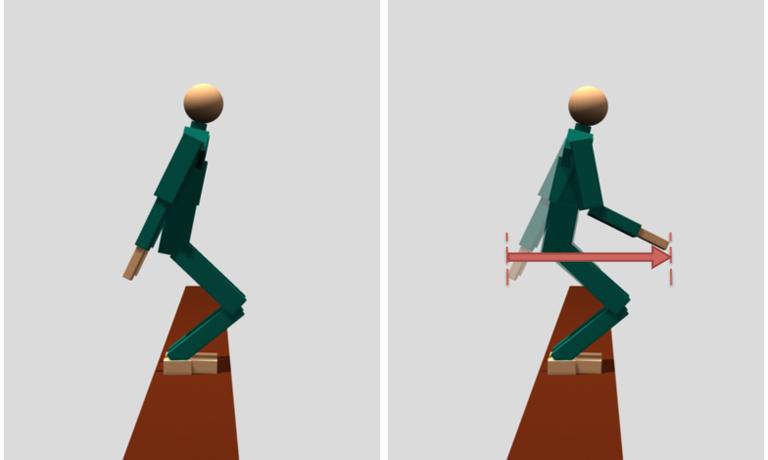
\includegraphics[width=0.58\textwidth]{images/intro_teach.png}
  \end{center}
   \vspace{-25pt}
  \caption{The proposed learning frame uses human readable instructions
    to teach motions.}
  \label{fig:intro_teach}
   \vspace{-10pt}
\end{wrapfigure}
In Chapter 5, I will describe an iterative framework to design dynamic
controllers using high-level, human-readable instructions,
inspired by a training process of athletes that consists of
interactive coaching and repetitive practices (\figref{intro_teach})
To enable interactive coaching, I introduce ``control rigs'' as
an intermediate layer of control module to facilitate the mapping between
human instructions and low-level control parameters.
During the practicing stage, control parameters are efficiently determined
using CMA-ES, which will be further improved in the following chapters.
The details of controllers development process using our iterative learning
framework will be shown with example parkour motions.

\subsection{Optimization with Failure Learning}
% Goal, Method (Strength), Verification + Image
A controller with many user constraints is difficult to optimize due to the
relatively small feasible region.
In Chapter 6, I will describe a new optimization algorithm for
highly-constrained problems based on the observation of human’s ability 
to learn from failure.
The proposed algorithm, CMA-C (Covariance Matrix Adaptation with
Classification) utilizes the failed simulation trials to approximate 
an infeasible region in the space of control rig parameters 
so that it can predict the quality of the samples,
resulting a faster convergence than the standard CMA-ES.

\subsection{Optimization for Parametrized Motor Skills}
% Goal, Method (Strength), Verification + Image
In Chapter 7, I will explain the optimization of parametrized motor skills.
The parametrization of the learned motor skills is an essential ability
because a robot can reinterpret the skill to a new situation, without
learning from scratch.
Instead of maintaining a single Gaussian distribution, 
the algorithm reduces the number of samples by evolving a parametrized
probability distribution for a range of skills.
I will test the algorithm on a simulated humanoid
robot learning three parametrized dynamic motor skills, 
including vertical jump, kick a ball, and walk.

\section{Model-based Learning for Virtual and Real Characters}
% Goal, Method (Strength), Verification + Images
\begin{wrapfigure}{l}{0.5\textwidth}
 \vspace{-10pt}
  \begin{center}
    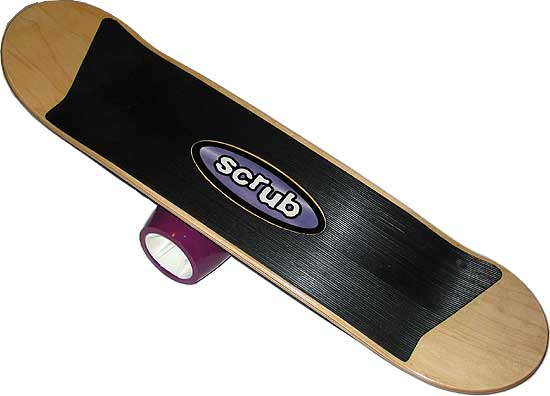
\includegraphics[width=0.48\textwidth]{images/intro_bongo.jpg}
  \end{center}
   \vspace{-25pt}
  \caption{Bongo Board balance toy.}
  \label{fig:intro_bongo}
   \vspace{-10pt}
\end{wrapfigure}
In Chapter 8, I will describe an iterative approach for for learning 
hardware models and optimizing control policies with 
as few hardware experiments as possible.
Instead of learning hardware models from scratch, the proposed approach only
learns the difference from a simulation model.
Similarly to the previous work, Gaussian Process is used to model 
the difference between dynamics of virtual and real characters
based on the collected hardware data.
To prove the concept, I will validate the algorithm on two different 
simulation models, one with perfect contacts and one with realistic contacts,
by finding a balancing controller for a bipedal robot on a bongo board
(\figref{intro_bongo}).

\section{Contributions}
The control and optimization methods discussed in this dissertation provide
several contributions to the computer animation community. 
These contributions are as follows:


\begin{itemize}
\item \textbf{A falling and landing strategy for virtual characters}
  The falling strategy presented in the dissertation allows the character to
  fall from a wide range of heights and initial speeds, continuously roll 
  on the ground, and get back on its feet, without inducing large stress on
  joints at any moment.
\item \textbf{A multiple contact falling strategy for robots}
  I also introduce a new falling strategy that can optimize a sequence
  of contacts, which optimizes the number and locations of contacts
  for the given initial state.
\item \textbf{An iterative learning framework for dynamic motor skills}
  Unlikely previous monolithic design processes in the literature,
  I proposed an iterative and interactive learning framework 
  using human readable instructions.
  Starting from a basic controller, the proposed framework allows a user 
  to easily train complex dynamic motion controllers within minutes,
  with only a few high-level instructions from the user.
\item \textbf{An optimization technique for highly constrained problems}
  I introduce a novel efficient optimization algorithm, CMA-C, that is 
  designed for the problem with many constraints and smaller feasible regions.
  The algorithm converges faster than the standard CMA-ES,
  by approximating the infeasible region using
  Supported Vector Machines.
\item \textbf{An optimization technique for parametrized tasks}
  I introduce an efficient evolutionary optimization algorithm for learning
  parametrized skills to achieve whole-body dynamic tasks, which is much
  faster than the baseline algorithm, CMA-ES.
\item \textbf{A model-based policy search for reducing hardware experiments}
  I propose an iterative approach for learning hardware model and optimizing
  policies with as few hardware experiments as possible by learning the
  difference between a simulation model and hardware.
\end{itemize}

\rule{\textwidth}{1pt}

In the next chapter, I will discuss the related work conducted by other
researchers to address similar problems.
